\documentclass[10pt]{article}

\usepackage{float}
\usepackage[T1]{fontenc}
\usepackage[utf8]{inputenc}
\usepackage[english]{babel}
\usepackage{amssymb,amsfonts,amsmath,amsthm}
\usepackage{graphicx}
\usepackage{lmodern}
\usepackage{mdframed}
\usepackage{hyperref}
\usepackage{cases}
\usepackage{framed}
\usepackage{pdfpages}
\usepackage{multicol}
\usepackage[margin=60pt]{geometry}
\usepackage{abstract}
\usepackage{caption}

\usepackage{pgfplots}
\pgfplotsset{every axis/.append style={line width=1pt}}

\definecolor{RED}{HTML}{EB6231}
\definecolor{YELLOW}{HTML}{E29D26}
\definecolor{BLUE}{HTML}{5D80B4}
\definecolor{LIGHTGREEN}{HTML}{6ABD9B}
\definecolor{GREEN}{HTML}{8FB03E}
\definecolor{PURPLE}{HTML}{BE1E2D}
\definecolor{BROWN}{HTML}{A97C50}
\definecolor{PINK}{HTML}{DA1C5C}

\newcommand{\R}{\textcolor{GREEN}{R}}

\definecolor{color1}{HTML}{EB6231}
\definecolor{color2}{HTML}{E29D26}
\definecolor{color3}{HTML}{5D80B4}
\definecolor{color4}{HTML}{6ABD9B}
\definecolor{color4}{HTML}{8FB03E}

\begin{document}

\begin{figure*}[hbt!]
 	\centering
 	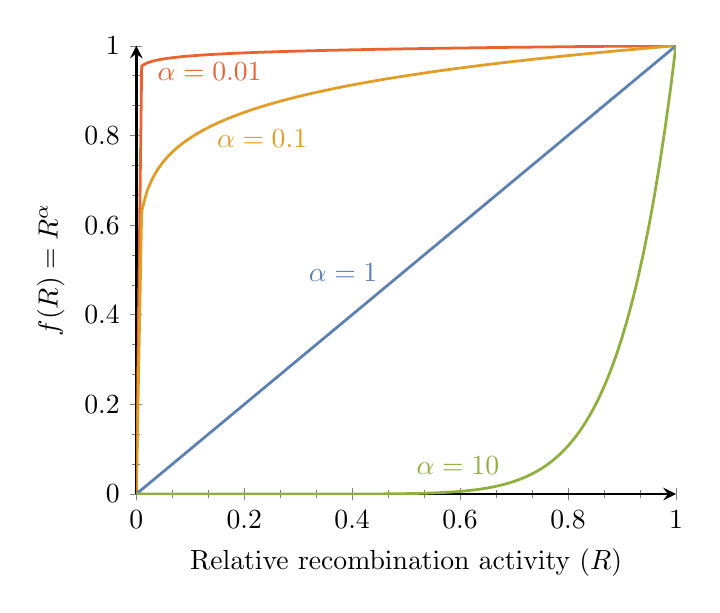
\begin{tikzpicture}
 	\begin{axis}[
 	ylabel={$f(R)= R^{\alpha}$},
 	xlabel={Relative recombination activity ($R$)},
 	domain=0:1,
 	samples=101,
 	minor tick num=2,
 	axis x line=bottom,
 	axis y line=left,
 	]
 	\addplot[color1]{x^(0.01)};
 	\addplot[color2]{x^(0.1)};
 	\addplot[color3]{x^(1)};
 	\addplot[color4]{x^(10)};
 	\node at (axis cs:0.02,0.90) [anchor=south west, color1] {$\alpha=0.01$};
 	\node at (axis cs:0.13,0.75) [anchor=south west, color2] {$\alpha=0.1$};
 	\node at (axis cs:0.3,0.45) [anchor=south west, color3] {$\alpha=1$};
 	\node at (axis cs:0.5,0.02) [anchor=south west, color4] {$\alpha=10$};
 	
 	\end{axis}
 	\end{tikzpicture}
 	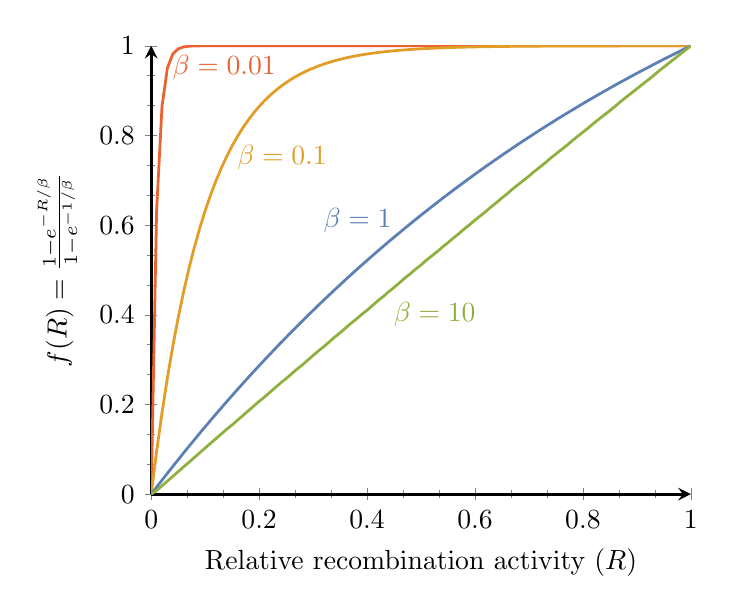
\begin{tikzpicture}
 	\begin{axis}[
 	ylabel={$f(R)= \tfrac{1 - e^{-R/ \beta}}{1 - e^{-1/ \beta}}$},
 	xlabel={Relative recombination activity ($R$)},
 	domain=0:1,
 	samples=101,
 	minor tick num=2,
 	axis x line=bottom,
 	axis y line=left,
 	]
 	\addplot[color1]{(1-exp(-x/0.01))/(1-exp(-1/0.01))};
 	\addplot[color2]{(1-exp(-x/0.1))/(1-exp(-1/0.1))};
 	\addplot[color3]{(1-exp(-x/1))/(1-exp(-1/1))};
 	\addplot[color4]{(1-exp(-x/10))/(1-exp(-1/10))};
  	\node at (axis cs:0.02,0.90) [anchor=south west, color1] {$\beta=0.01$};
  	\node at (axis cs:0.14,0.70) [anchor=south west, color2] {$\beta=0.1$};
  	\node at (axis cs:0.3,0.56) [anchor=south west, color3] {$\beta=1$};
  	\node at (axis cs:0.43,0.35) [anchor=south west, color4] {$\beta=10$};
  	
 	\end{axis}
 	\end{tikzpicture}
 	\caption{$f$ as a function of the recombination activity $R$, in the case of a power-law function (left panel) and in the case of an exponential function (right panel).\label{fig:fitness}}
\end{figure*}
\begin{figure*}[hbt!]
  	\centering
  	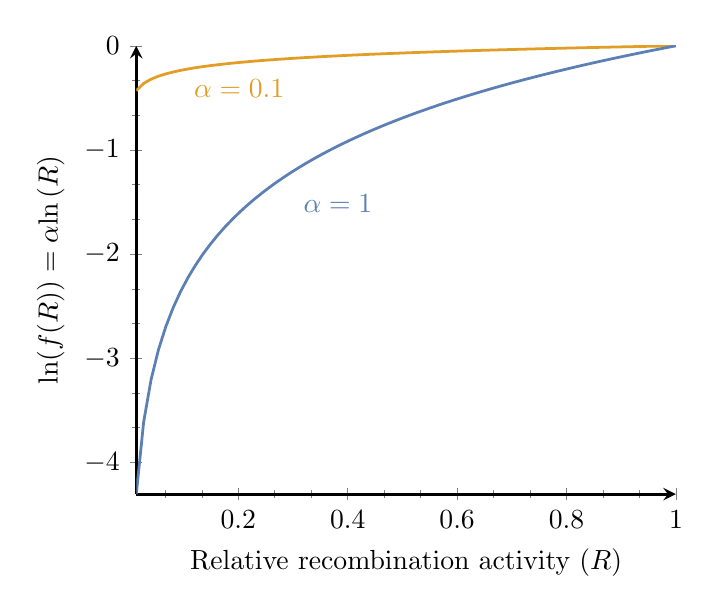
\begin{tikzpicture}
  	\begin{axis}[
  	ylabel={$\mathrm{ln}(f(R))= \alpha \mathrm{ln} \left( R \right)$},
  	xlabel={Relative recombination activity ($R$)},
  	domain=0:1,
  	samples=75,
  	minor tick num=2,
  	axis x line=bottom,
  	axis y line=left,
  	]
  	\addplot[color2]{ln(x^(0.1))};
  	\addplot[color3]{ln(x^(1))};
  	\node at (axis cs:0.1,-0.6) [anchor=south west, color2] {$\alpha=0.1$};
  	\node at (axis cs:0.3,-1.7) [anchor=south west, color3] {$\alpha=1$};
  	
  	\end{axis}
  	\end{tikzpicture}
  	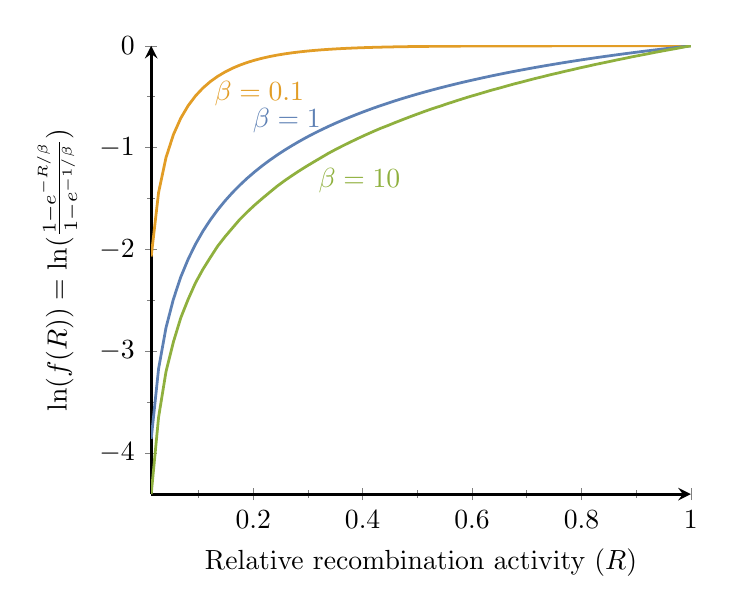
\begin{tikzpicture}
  	\begin{axis}[
  	ylabel={$\mathrm{ln}(f(R))= \mathrm{ln} ( \tfrac{1 - e^{-R/ \beta}}{1 - e^{-1/ \beta}} )$},
  	xlabel={Relative recombination activity ($R$)},
  	domain=0:1,
  	samples=75,
  	minor tick num=1,
  	axis x line=bottom,
  	axis y line=left,
  	]
  	\addplot[color2]{ln((1-exp(-x/0.1))/(1-exp(-1/0.1)))};
  	\addplot[color3]{ln((1-exp(-x/1))/(1-exp(-1/1)))};
  	\addplot[color4]{ln((1-exp(-x/10))/(1-exp(-1/10)))};
	\node at (axis cs:0.11,-0.69) [anchor=south west, color2] {$\beta=0.1$};
	\node at (axis cs:0.18,-0.96) [anchor=south west, color3] {$\beta=1$};
	\node at (axis cs:0.30,-1.55) [anchor=south west, color4] {$\beta=10$};

  	\end{axis}
  	\end{tikzpicture}
  	\caption{$\mathrm{ln}(f(R))$ as a function of the recombination activity $R$, in the case of a power-law function (left panel) and in the case of an exponential function (right panel).\label{fig:logfitness}}
\end{figure*}
\begin{figure*}[hbt!]
	\centering
  	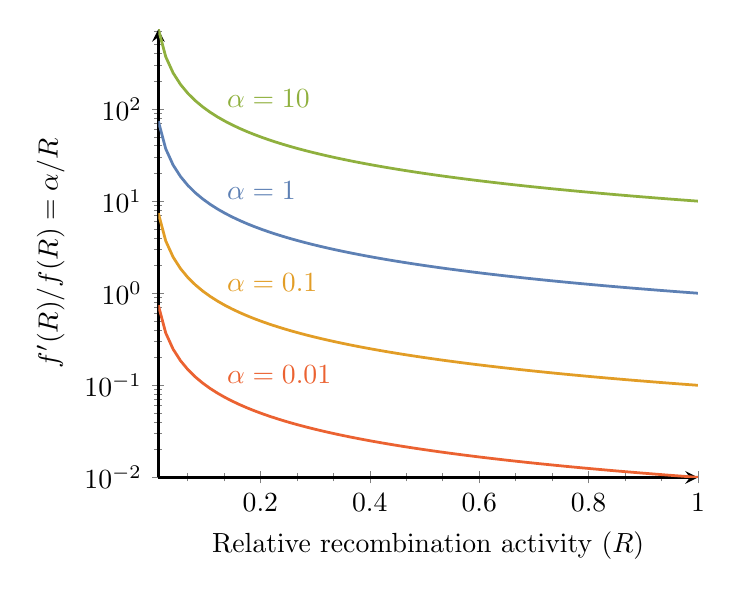
\begin{tikzpicture}
  	\begin{axis}[
  	ylabel={$f'(R) / f(R)= \alpha / R$},
  	xlabel={Relative recombination activity ($R$)},
  	domain=0:1,
  	samples=75,
  	minor tick num=2,
  	axis x line=bottom,
  	axis y line=left,
  	ymode = log,
  	]
  	\addplot[color1]{(0.01 / x)};
  	\addplot[color2]{(0.1 / x)};
  	\addplot[color3]{(1 / x)};
  	\addplot[color4]{(10 / x)};
  	\node at (axis cs:0.12,0.08) [anchor=south west, color1] {$\alpha=0.01$};
  	\node at (axis cs:0.12,0.8) [anchor=south west, color2] {$\alpha=0.1$};
  	\node at (axis cs:0.12,8) [anchor=south west, color3] {$\alpha=1$};
  	\node at (axis cs:0.12,80) [anchor=south west, color4] {$\alpha=10$};
  	
  	\end{axis}
  	\end{tikzpicture}
	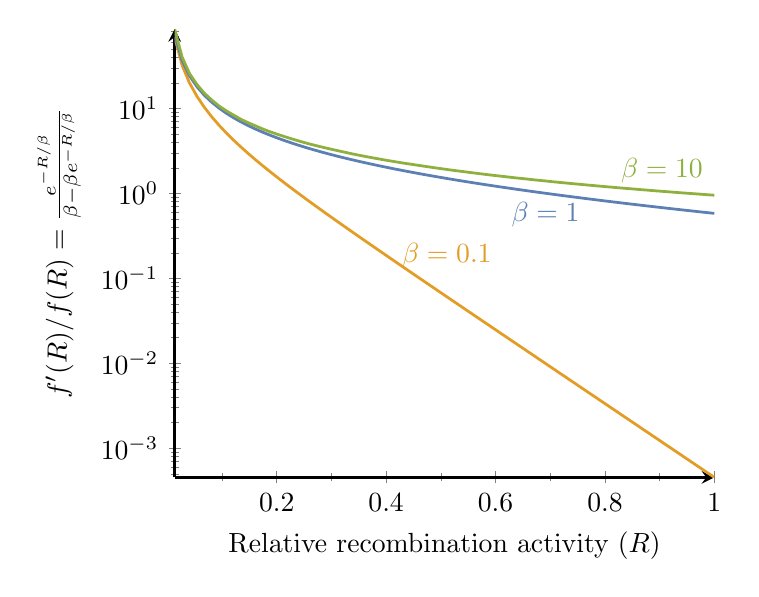
\begin{tikzpicture}
	\begin{axis}[
	ylabel={$f'(R) / f(R)=  \tfrac{ e^{-R/ \beta}}{ \beta  - \beta e^{-R/ \beta} } $},
	xlabel={Relative recombination activity ($R$)},
	domain=0:1,
	samples=75,
	minor tick num=1,
	axis x line=bottom,
	axis y line=left,
	ymode = log,
	]
	\addplot[color2]{exp(-x/0.1)/(0.1*(1-exp(-x/0.1)))};
	\addplot[color3]{exp(-x/1)/(1*(1-exp(-x/1)))};
	\addplot[color4]{exp(-x/10)/(10*(1-exp(-x/10)))};
	\node at (axis cs:0.41,0.1) [anchor=south west, color2] {$\beta=0.1$};
	\node at (axis cs:0.61,0.3) [anchor=south west, color3] {$\beta=1$};
	\node at (axis cs:0.81,1) [anchor=south west, color4] {$\beta=10$};
	
	\end{axis}
	\end{tikzpicture}
	\caption{$f'(R)/f(R)=\mathrm{ln}(f(R))'$ as a function of the recombination activity $R$, in the case of a power-law function (left panel) and in the case of an exponential function (right panel).\label{fig:dlogfitness}}
\end{figure*}
\begin{figure*}[hbt!]
	\centering
	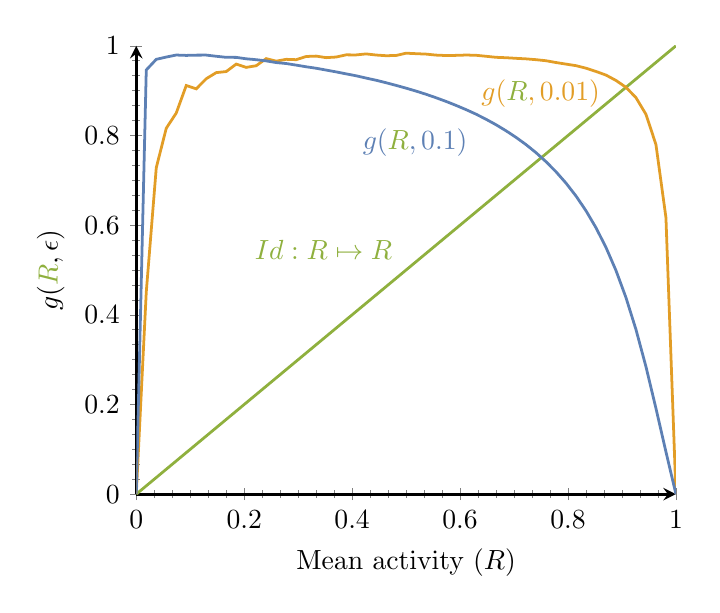
\begin{tikzpicture}
	\begin{axis}[
	ylabel={$g(\R, \epsilon)$},
	xlabel={Mean activity ($R$)},
	domain=0:1,
	samples=55,
	minor tick num=5,
	axis x line=bottom,
	axis y line=left,
	]
	\addplot[GREEN]{x};
	\addplot[color2]{(1-exp(-0.01*2*x/(1-x)))/(0.01*2*x/(1-x))};
	\addplot[color3]{(1-exp(-0.1*2*x/(1-x)))/(0.1*2*x/(1-x))};;
	\node at (axis cs:0.2,0.5) [anchor=south west, GREEN] {$Id: \R \mapsto \R $};
	\node at (axis cs:0.62,0.84) [anchor=south west, color2] {$g(\R, 0.01)$};
	\node at (axis cs:0.4,0.73) [anchor=south west, color3] {$g(\R, 0.1)$};
	
	\end{axis}
	\end{tikzpicture}
	\captionsetup{labelformat=empty}
	\caption[]{Self-consistent solution as a fixed point, in the form $\R = g(\R, \epsilon)$}
\end{figure*}
\end{document}
